\chapter{Experimental Results and Performance Analysis}
\label{chap:experimental-results}

\section{System Reliability: Success vs. Failure Analysis}

All four direct attestation scenarios completed successfully in all 10 measured
iterations, and the three ML-DSA plus ECDSA host-side prequote scenarios also
completed successfully in all 10 measured iterations
(table~\ref{tab:reliability-summary}).

\begin{table}[t]
\centering
\small
\caption{Measured scenario reliability.}
\label{tab:reliability-summary}
\begin{tabular}{|l|l|r|r|l|}
\hline
Scenario & Execution context & Successes & Failures & Failure stage \\
\hline
ECDSA direct & guest TDX full flow & 10 & 0 & --- \\
ML-DSA-44 direct & guest TDX full flow & 10 & 0 & --- \\
ML-DSA-65 direct & guest TDX full flow & 10 & 0 & --- \\
ML-DSA-87 direct & guest TDX full flow & 10 & 0 & --- \\
ECDSA wrapper & host SGX prequote & 10 & 0 & --- \\
ML-DSA-44 wrapper & host SGX prequote & 10 & 0 & --- \\
ML-DSA-65 wrapper & host SGX prequote & 10 & 0 & --- \\
ML-DSA-87 wrapper & host SGX prequote & 10 & 0 & --- \\
\hline
\end{tabular}
\end{table}

The ECDSA wrapper failure reported in earlier experiments is no longer present
in the updated dataset. In the current host environment, the stock host-side
prequote API path completed successfully in all 10 measured iterations, so the
wrapper baseline can now be compared directly with the ML-DSA wrapper
scenarios.

\section{Dimensional Analysis: Quote Size Expansion}

Using the ECDSA baseline \(|Q_{\mathrm{ECDSA}}| = 5006\) bytes, the observed
direct quote-size expansion ratios were
(table~\ref{tab:direct-dimensional-analysis}):
\[
  \frac{|Q_{44}|}{|Q_{\mathrm{ECDSA}}|} = 1.767,
  \qquad
  \frac{|Q_{65}|}{|Q_{\mathrm{ECDSA}}|} = 2.073,
  \qquad
  \frac{|Q_{87}|}{|Q_{\mathrm{ECDSA}}|} = 2.464.
\]

\begin{table}[t]
\centering
\small
\caption{Direct-path quote and collateral sizes.}
\label{tab:direct-dimensional-analysis}
\begin{tabular}{|l|r|r|r|}
\hline
Algorithm & Quote size [B] & Collateral size [B] & Quote expansion vs.\ ECDSA \\
\hline
ECDSA P-256 & 5006 & 14355 & 1.000 \\
ML-DSA-44 & 8847 & 14388 & 1.767 \\
ML-DSA-65 & 10376 & 14388 & 2.073 \\
ML-DSA-87 & 12334 & 14388 & 2.464 \\
\hline
\end{tabular}
\end{table}

Two facts follow immediately from the results. First, the quote-size overhead
grows monotonically with the ML-DSA parameter set. Second, the verifier-side
collateral size is essentially constant across the PQC scenarios; the measured
collateral expansion relative to ECDSA was only \(1.00230\times\).

This second point is important: the additional dimensional cost of the PQC
scenarios is carried almost entirely by the quote itself, not by the
verification collateral bundle. The reason is structural. In all four direct
scenarios, the TDX quote still contains the same fixed-format components: the
quote header, the TD report body, the authentication-data wrapper, and the
certification-data wrapper. The part that changes materially with the
algorithm is the attestation-key-specific payload, namely the embedded
attestation public key and the signature data.

Consequently, the monotonic sequence
\[
  |Q_{44}| < |Q_{65}| < |Q_{87}|
\]
reflects the strictly increasing ML-DSA parameter sizes. From a security
perspective, this is the first explicit trade-off exposed by the measurements:
ML-DSA-44 is the smallest of the tested PQC parameter sets, ML-DSA-65 is
intermediate, and ML-DSA-87 is the largest and most conservative one; the
dimensional cost increases accordingly. The same monotonic growth remains
visually immediate in the plotted direct-path comparison
(figure~\ref{fig:quote-size-comparison}).

\begin{figure}[t]
\centering
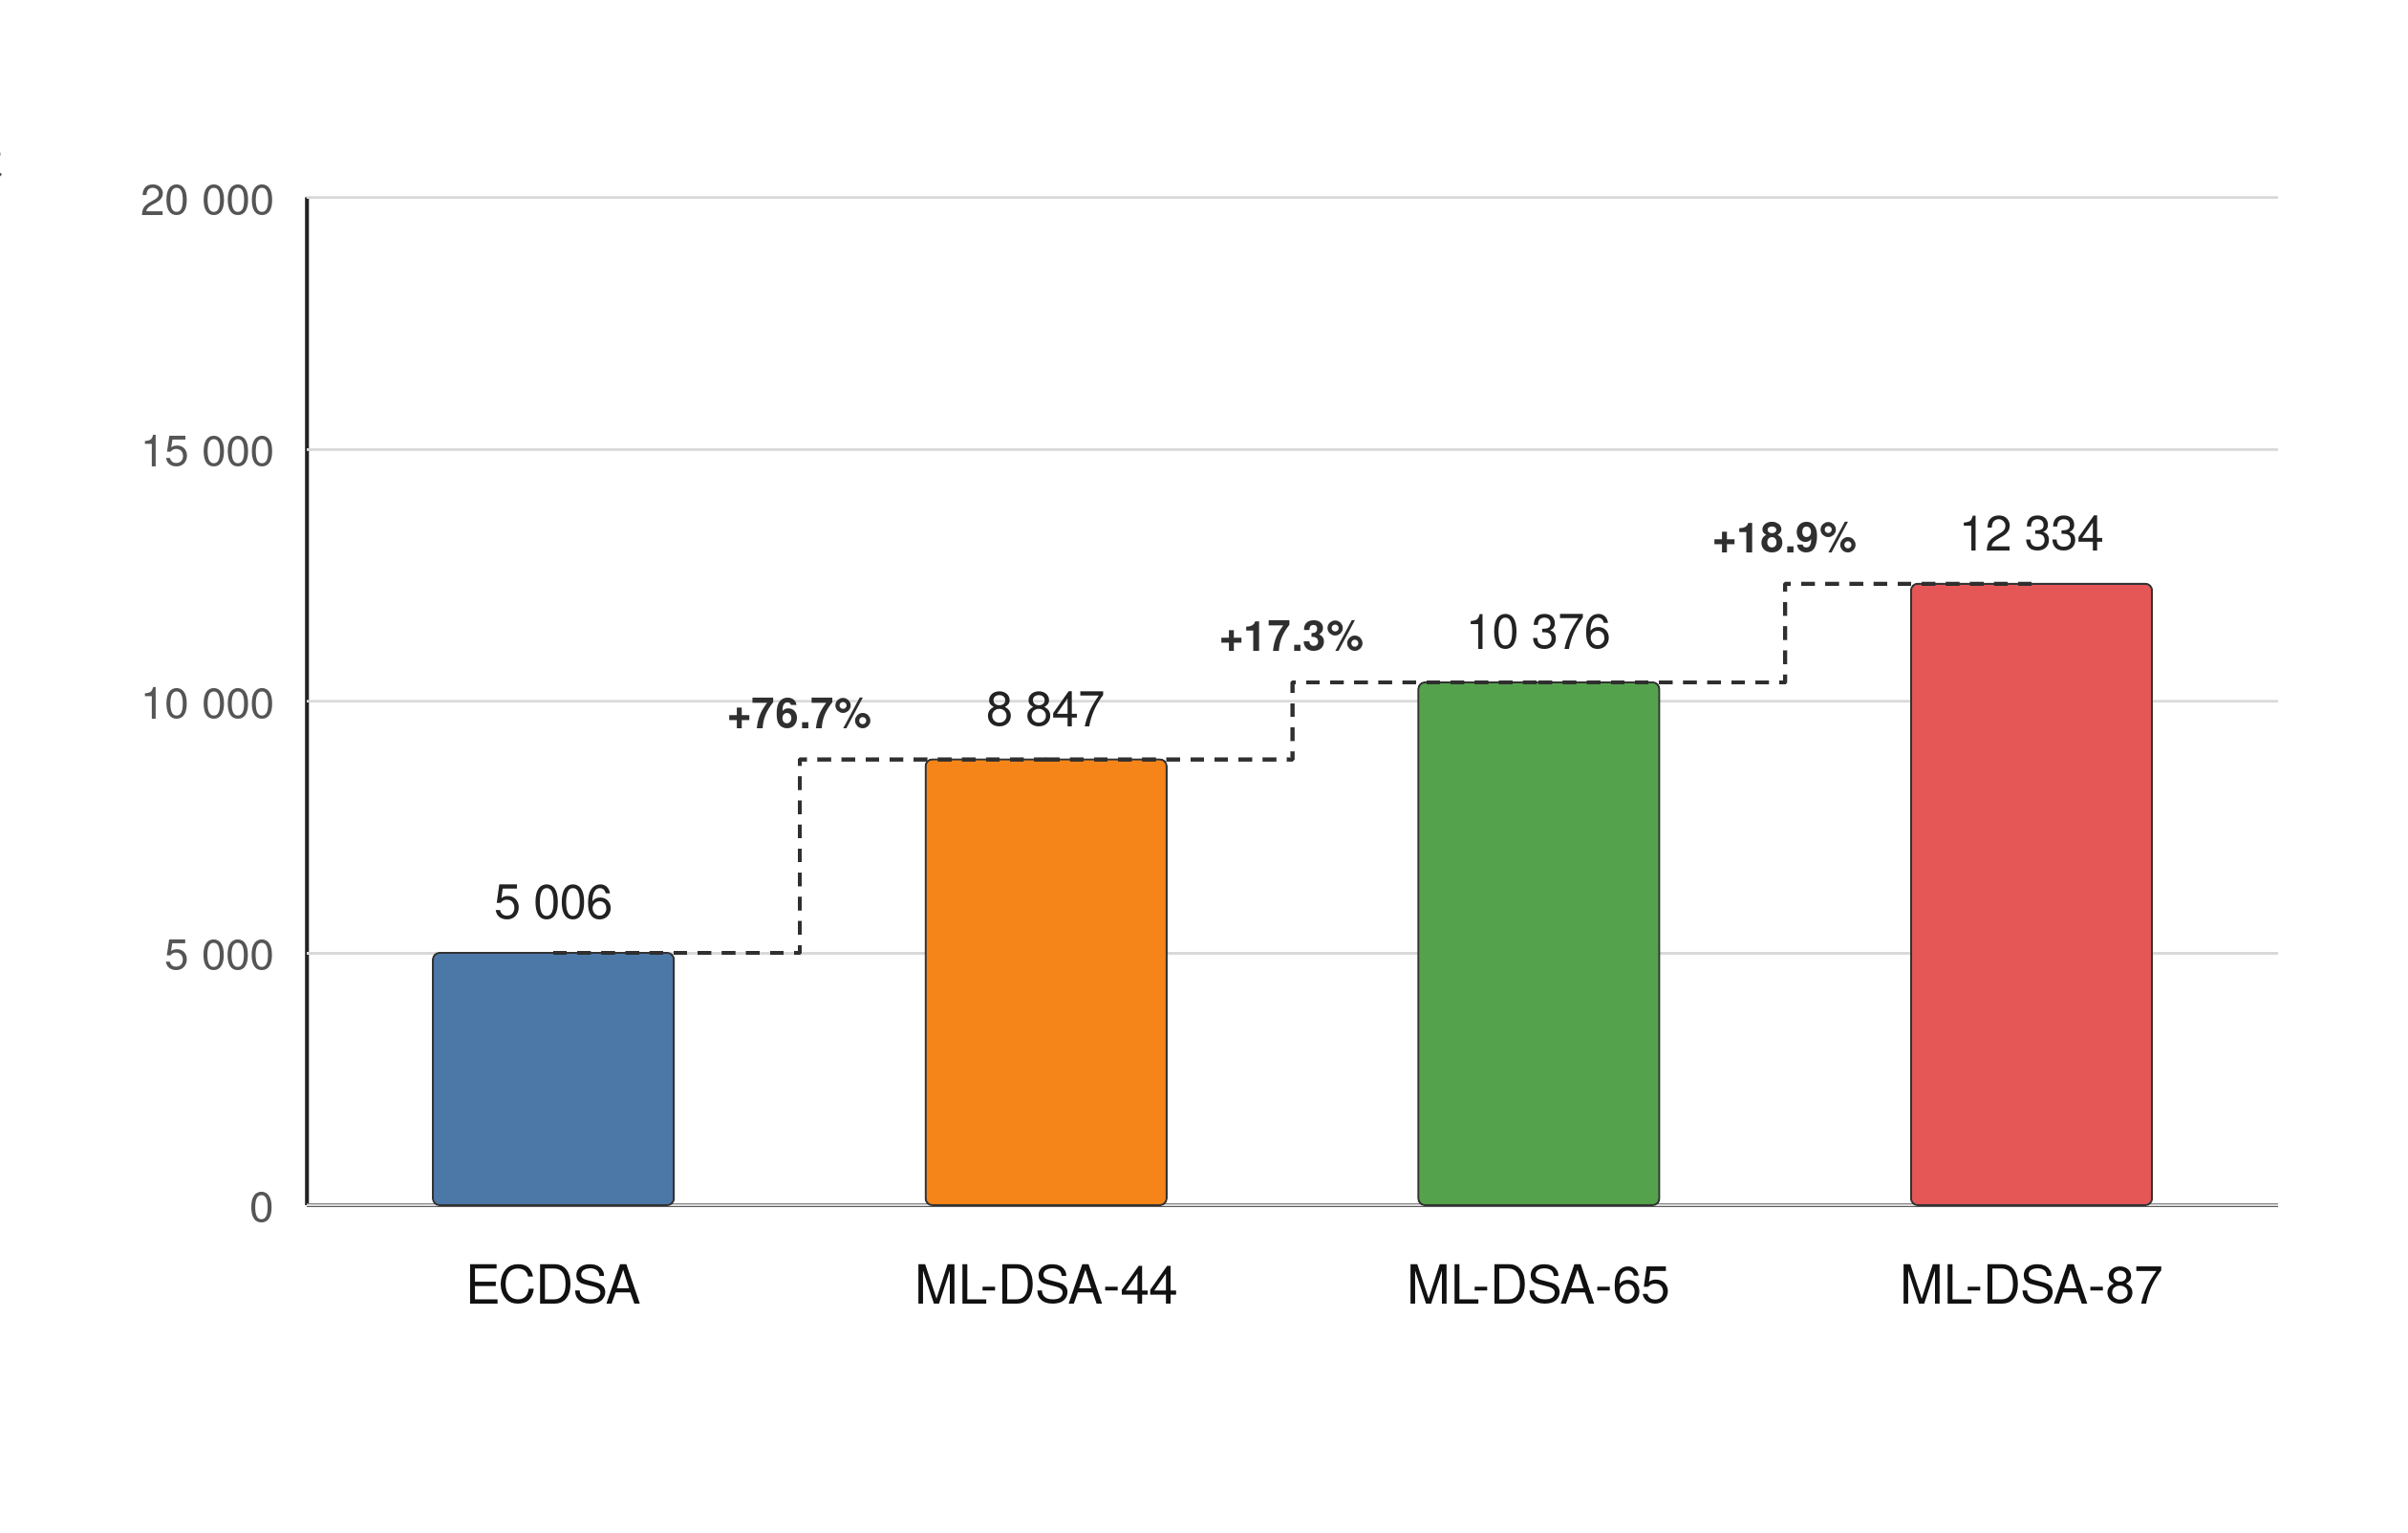
\includegraphics[width=0.88\linewidth]{figures/generated/quote_size_comparison.png}
\caption{Direct-path quote-size comparison across ECDSA and the three ML-DSA parameter sets.}
\label{fig:quote-size-comparison}
\end{figure}

The host-side prequote path returned the corresponding \emph{required quote
buffer sizes} produced by \texttt{tee\_att\_get\_quote\_size()} before any
final quote serialization or verifier-side collateral retrieval
(table~\ref{tab:wrapper-quote-sizes}).

\begin{table}[t]
\centering
\small
\caption{Host-side prequote required quote-buffer sizes.}
\label{tab:wrapper-quote-sizes}
\begin{tabular}{|l|r|}
\hline
Algorithm & Required quote buffer size [B] \\
\hline
ECDSA P-256 & 5243 \\
ML-DSA-44 & 5573 \\
ML-DSA-65 & 7102 \\
ML-DSA-87 & 9060 \\
\hline
\end{tabular}
\end{table}

These wrapper-side values must not be interpreted as the serialized quote sizes
observed on the direct guest-side attestation path. They are allocation sizes
returned by the prequote API. This distinction explains the apparently
counter-intuitive ECDSA result: the wrapper path returned 5243~B, while the
direct hardware path produced an actual quote of 5006~B. There is no
contradiction here. The two numbers refer to different objects. The direct
measurement reports the emitted quote bytes, whereas the prequote measurement
reports the buffer budget required by the wrapper. In the measured ECDSA direct
scenario, the emitted quote was a version-4 quote; by contrast, the wrapper
size computation follows a larger quote-structure budget on the host side.

\section{Execution Costs (Latency and CPU Cycles)}

\subsection{Context Creation and Init\_quote}

The host-side prequote benchmark is the only configuration that measures
\texttt{tee\_att\_create\_context()} and \texttt{tee\_att\_init\_quote()}
without folding them into the guest TDX path
(table~\ref{tab:wrapper-latency}).

\begin{table}[t]
\centering
\small
\caption{Host-side prequote execution costs.}
\label{tab:wrapper-latency}
\begin{tabular}{|l|r|r|r|r|}
\hline
Algorithm & Context create & Init\_quote full & Quote-size query & End-to-end \\
 & [\(\mu s\) / Mcycles] & [ms / Mcycles] & [ms / Mcycles] & [ms / Mcycles] \\
\hline
ECDSA P-256 & 36.492 / 0.106 & 22.593 / 65.518 & 0.080 / 0.231 & 22.710 / 65.858 \\
ML-DSA-44 & 51.681 / 0.150 & 15.532 / 45.041 & 8.697 / 25.221 & 24.281 / 70.416 \\
ML-DSA-65 & 66.840 / 0.194 & 21.184 / 61.433 & 9.558 / 27.719 & 30.810 / 89.350 \\
ML-DSA-87 & 62.819 / 0.182 & 21.305 / 61.784 & 9.165 / 26.579 & 30.534 / 88.549 \\
\hline
\end{tabular}
\end{table}

The data show that context creation is negligible compared to the enclave-side
prequote initialization work: it remains on the order of \(10^{-4}\) seconds
and approximately \(10^{5}\) cycles in all four wrapper variants, whereas
\texttt{init\_quote\_full} stays in the range of roughly 15--23~ms and
45--66~million cycles.

The absence of a clean monotonic ordering across the ML-DSA variants in this
prequote stage is expected. The measured \texttt{init\_quote\_full} path is
dominated by wrapper and enclave-management logic that is mostly independent of
the final signature size. In other words, this stage measures SGX-host
control-path work more than pure algorithm-dependent signing work.

\subsection{Quote-size Retrieval Overhead}

The host-side prequote benchmark also isolates the cost of
\texttt{tee\_att\_get\_quote\_size()}. The measured mean latency is between
8.697~ms and 9.558~ms for the ML-DSA scenarios, while the ECDSA wrapper shows
a much lower mean of about 0.080~ms.

This difference is important, but it must be interpreted correctly. The
ECDSA wrapper does \emph{not} generate a much smaller final quote than the PQC
variants at this stage; it only answers the buffer-size query much more
quickly. The quote-size query is therefore not a negligible bookkeeping
operation in the PQC configuration, whereas it is close to negligible in the
stock ECDSA wrapper path.

\subsection{Quote Generation and Rejection Sampling Impact}

The direct-path quote-generation stage was measured by timing
\texttt{tdx\_att\_get\_quote()} after a successful
\texttt{tdx\_att\_get\_report()}. The measured means are:

\begin{itemize}
  \item ECDSA: 4.068 ms and 11.796 Mcycles;
  \item ML-DSA-44: 12.902 ms and 37.411 Mcycles;
  \item ML-DSA-65: 12.926 ms and 37.481 Mcycles;
  \item ML-DSA-87: 13.386 ms and 38.814 Mcycles.
\end{itemize}

Relative to ECDSA, the quote-generation latency ratios were:
\[
  \frac{T^{\mathrm{quote}}_{44}}{T^{\mathrm{quote}}_{\mathrm{ECDSA}}} = 3.171,
  \qquad
  \frac{T^{\mathrm{quote}}_{65}}{T^{\mathrm{quote}}_{\mathrm{ECDSA}}} = 3.177,
  \qquad
  \frac{T^{\mathrm{quote}}_{87}}{T^{\mathrm{quote}}_{\mathrm{ECDSA}}} = 3.290.
\]

These values quantify the complete signing-side cost of the experimental PQC
path. They do not isolate internal ML-DSA rejection iterations with a
dedicated counter. Consequently, the measured quote-generation overhead must
be interpreted as the aggregate effect of the full ML-DSA signing path inside
the quote-generation routine, including rejection sampling, key-material
handling, and quote-structure assembly.

Within the PQC family, the difference between ML-DSA-44, ML-DSA-65, and
ML-DSA-87 is now more visible than in the earlier dataset: ML-DSA-87 is the
slowest variant, while ML-DSA-44 and ML-DSA-65 remain very close to one
another among the three PQC settings. The principal monotonic effect of moving from ML-DSA-44 to
ML-DSA-87 is therefore still dimensional, but the runtime gap is no longer
negligible.

\subsection{Verification Latency}

The direct verifier stage was measured by timing
\texttt{tdx\_qv\_verify\_quote()} after the collateral bundle had already been
retrieved. The measured means were:

\begin{itemize}
  \item ECDSA: 11.783 ms and 34.169 Mcycles;
  \item ML-DSA-44: 13.660 ms and 39.613 Mcycles;
  \item ML-DSA-65: 13.462 ms and 39.038 Mcycles;
  \item ML-DSA-87: 13.598 ms and 39.433 Mcycles.
\end{itemize}

The corresponding ratios relative to ECDSA were \(1.159\times\) for
ML-DSA-44, \(1.142\times\) for ML-DSA-65, and \(1.154\times\) for
ML-DSA-87. The direct cryptographic verification cost therefore increased
moderately across all PQC parameter sets.

That ML-DSA-44, ML-DSA-65, and ML-DSA-87 all lie in a narrow band should not
be interpreted as a universal algorithmic property. The measured stage is not
a bare signature-verification microbenchmark; it includes quote parsing,
certification-data interpretation, and the fixed verifier logic shared by all
scenarios. The result therefore indicates that the algorithm-dependent
verification work is not yet the dominant term of the integrated verifier
path.

This result matters because it sharply separates two effects: the
cryptographic verification cost of the quote, which remains in the low tens of
milliseconds, and the operational cost of the surrounding collateral path,
which is much larger in the current ML-DSA experimental configuration.

\section{End-to-End Flow Latency Analysis}

The direct-path stage means and the overall end-to-end cost are reported in
the measured results (table~\ref{tab:direct-latency}).

\begin{table}[t]
\centering
\small
\caption{Direct-path stage means.}
\label{tab:direct-latency}
\begin{tabular}{|l|r|r|r|r|}
\hline
Algorithm & Quote generation & Collateral fetch & Verification & End-to-end \\
 & [ms / Mcycles] & [ms / cycles] & [ms / Mcycles] & [ms / cycles] \\
\hline
ECDSA P-256 & 4.068 / 11.796 & 1.022 / 2.964M & 11.783 / 34.169 & 16.897 / 49.000M \\
ML-DSA-44 & 12.902 / 37.411 & 1425.423 / 4.134B & 13.660 / 39.613 & 1452.250 / 4.212B \\
ML-DSA-65 & 12.926 / 37.481 & 1393.169 / 4.040B & 13.462 / 39.038 & 1419.850 / 4.118B \\
ML-DSA-87 & 13.386 / 38.814 & 1393.247 / 4.040B & 13.598 / 39.433 & 1420.498 / 4.119B \\
\hline
\end{tabular}
\end{table}

The absolute end-to-end figures are dominated by different stages depending on
the scenario family. In the stock ECDSA baseline, verification itself accounts
for about 69.74\% of the total measured end-to-end time, while quote
generation accounts for about 24.08\%. In the ML-DSA scenarios, collateral
retrieval accounts for 98.15\% (ML-DSA-44), 98.12\% (ML-DSA-65), and 98.08\%
of the total measured end-to-end time.

This decomposition is more informative than the raw totals alone. The end-to-end ratios relative to ECDSA,
\[
  \frac{T^{\mathrm{e2e}}_{44}}{T^{\mathrm{e2e}}_{\mathrm{ECDSA}}} = 85.95,
  \qquad
  \frac{T^{\mathrm{e2e}}_{65}}{T^{\mathrm{e2e}}_{\mathrm{ECDSA}}} = 84.03,
  \qquad
  \frac{T^{\mathrm{e2e}}_{87}}{T^{\mathrm{e2e}}_{\mathrm{ECDSA}}} = 84.07,
\]
do not imply that ML-DSA signing or verification is intrinsically two orders
of magnitude slower than ECDSA. They show instead that, in the present
experimental deployment, the verifier-side collateral path for the private
TDQE-identity configuration dominates the flow. The cryptographic stages
themselves remain in the millisecond range.

This point must be interpreted carefully. The ML-DSA end-to-end path was
deliberately routed through the repository-local private TDQE-identity
configuration in order to exercise a complete DCAP API flow, including quote
generation, collateral retrieval, and final verifier acceptance with the
experimental TDQE identity override. That path is useful as a functional
end-to-end validation of the prototype, but it is not a good basis for a
fine-grained timing comparison against the stock ECDSA verifier path. In the
ML-DSA scenarios, the private collateral service path adds a large
infrastructure-specific delay that is not a direct property of the ML-DSA
signature algorithm itself. For this reason, the full end-to-end numbers should
be read primarily as proof that the complete PQC attestation flow works, not as
the most meaningful timing metric for comparing ML-DSA and ECDSA at the
algorithmic level.

This also explains why the end-to-end ordering is not monotonic in the same way as the quote-size ordering. If the signature algorithm were the dominant factor, one would expect
\[
  T^{\mathrm{e2e}}_{44} < T^{\mathrm{e2e}}_{65} < T^{\mathrm{e2e}}_{87}.
\]
The measurements do not follow this pattern because the largest component of
the end-to-end time is the collateral-retrieval stage, whose latency depends
on the verification path and remote collateral service behavior rather than on
the size of the ML-DSA signature itself. For this reason, the end-to-end
figures should be interpreted as system-level costs of the current prototype
deployment, not as pure algorithmic costs.

To isolate the algorithm-dependent portion of the integrated path more
accurately, it is more informative to subtract the collateral-fetch stage and
compare only report generation, quote generation, and verification
(figure~\ref{fig:end-to-end-latency-without-collateral}). Under this view, all
four scenarios remain in the low-millisecond regime, and the PQC overhead is
much smaller than the raw full end-to-end ratios suggest.

Formally, let
\[
  T^{\mathrm{e2e}\setminus\mathrm{coll}}_a
  =
  T^{\mathrm{e2e}}_a - T^{\mathrm{coll}}_a,
\]
where \(T^{\mathrm{coll}}_a\) is the measured collateral-fetch latency for
algorithm \(a\). Using this reduced metric, the measured means become
15.874~ms for ECDSA, 26.826~ms for ML-DSA-44, 26.681~ms for ML-DSA-65, and
27.251~ms for ML-DSA-87. The corresponding ratios relative to ECDSA are
\[
  \frac{T^{\mathrm{e2e}\setminus\mathrm{coll}}_{44}}
       {T^{\mathrm{e2e}\setminus\mathrm{coll}}_{\mathrm{ECDSA}}}
  = 1.690,
  \qquad
  \frac{T^{\mathrm{e2e}\setminus\mathrm{coll}}_{65}}
       {T^{\mathrm{e2e}\setminus\mathrm{coll}}_{\mathrm{ECDSA}}}
  = 1.681,
  \qquad
  \frac{T^{\mathrm{e2e}\setminus\mathrm{coll}}_{87}}
       {T^{\mathrm{e2e}\setminus\mathrm{coll}}_{\mathrm{ECDSA}}}
  = 1.717.
\]

These reduced ratios are far more representative of the practical
algorithm-dependent overhead than the raw \(84\times\) to \(86\times\)
full-flow ratios. They show that, once the private collateral path is removed
from the comparison, the end-to-end cost of the PQC scenarios is roughly
1.7 times the ECDSA baseline rather than two orders of magnitude larger. They
also confirm that ML-DSA-44 and ML-DSA-65 are nearly indistinguishable at this
integration level, while ML-DSA-87 remains the most expensive of the three
PQC settings.

\begin{figure}[t]
\centering
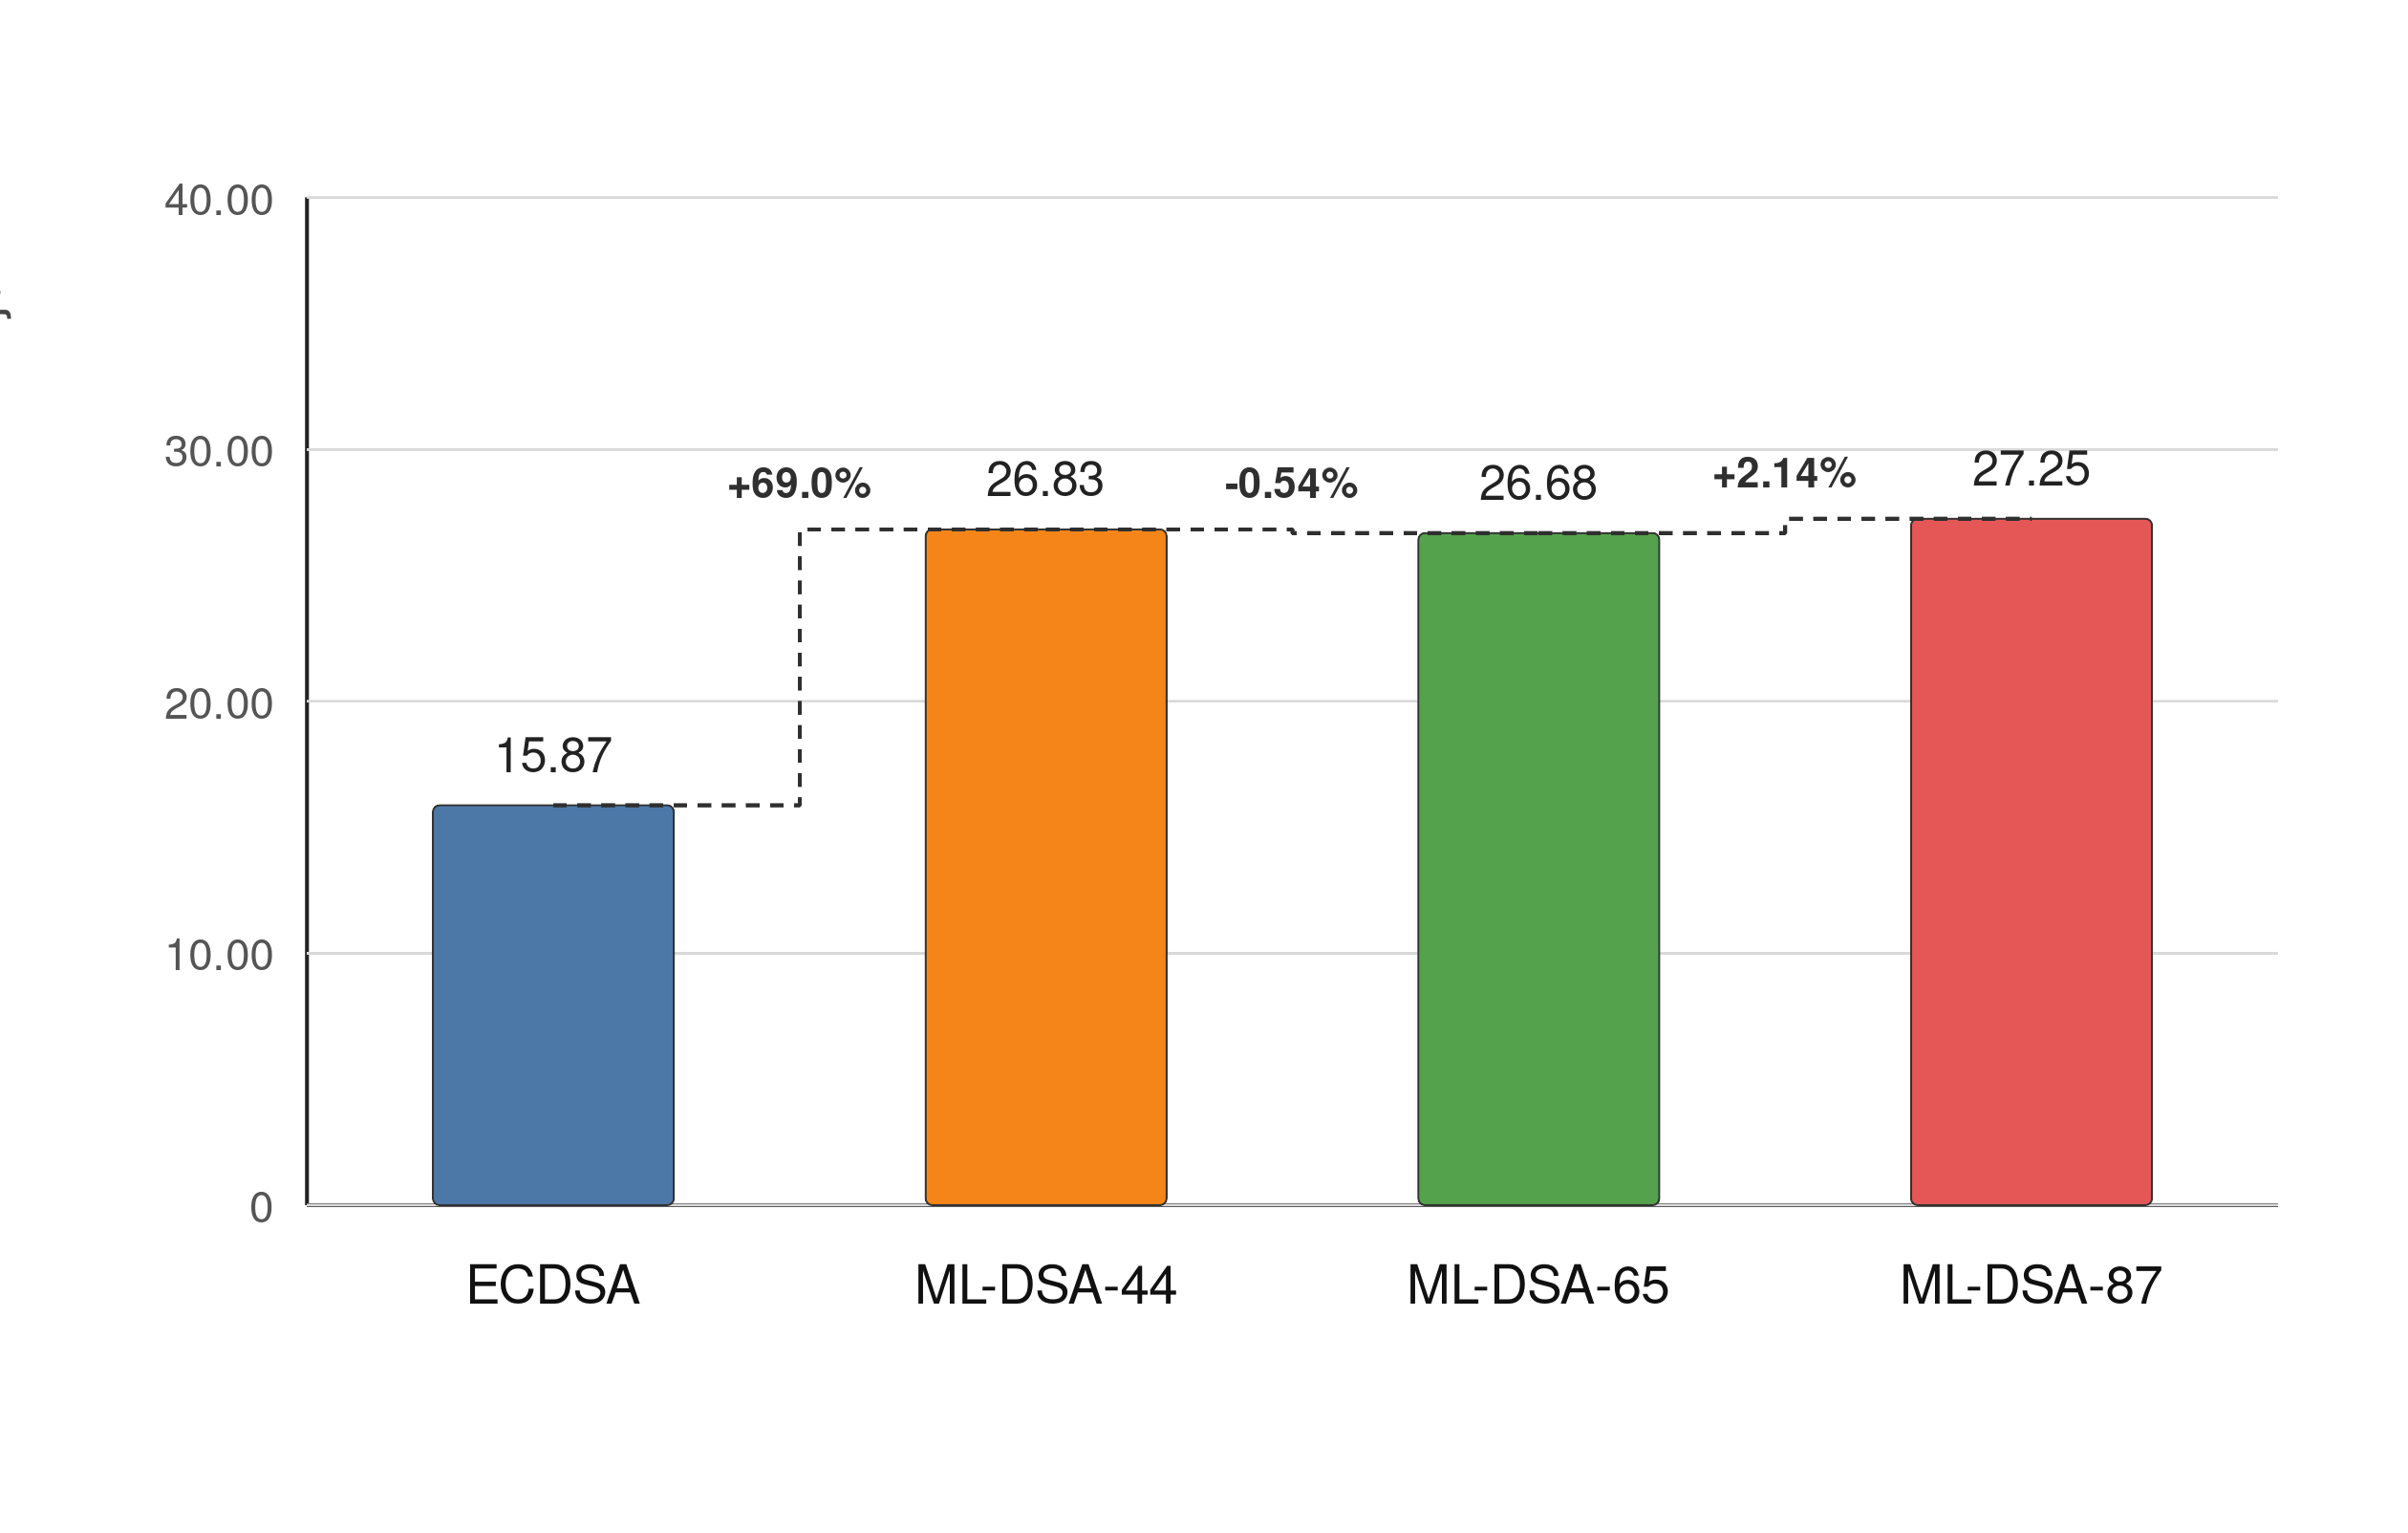
\includegraphics[width=0.90\linewidth]{figures/generated/end_to_end_latency_without_collateral.png}
\caption{End-to-end latency after removing the collateral-fetch stage.}
\label{fig:end-to-end-latency-without-collateral}
\end{figure}

The same decomposition can be expressed as a percentage contribution over the
reduced end-to-end total
(figure~\ref{fig:end-to-end-stage-share-without-collateral}). Once the
collateral-fetch stage is removed, quote generation and verification become the
dominant terms again, which is the correct perspective for discussing the
security-performance trade-off of the signature algorithms themselves.

\begin{figure}[t]
\centering
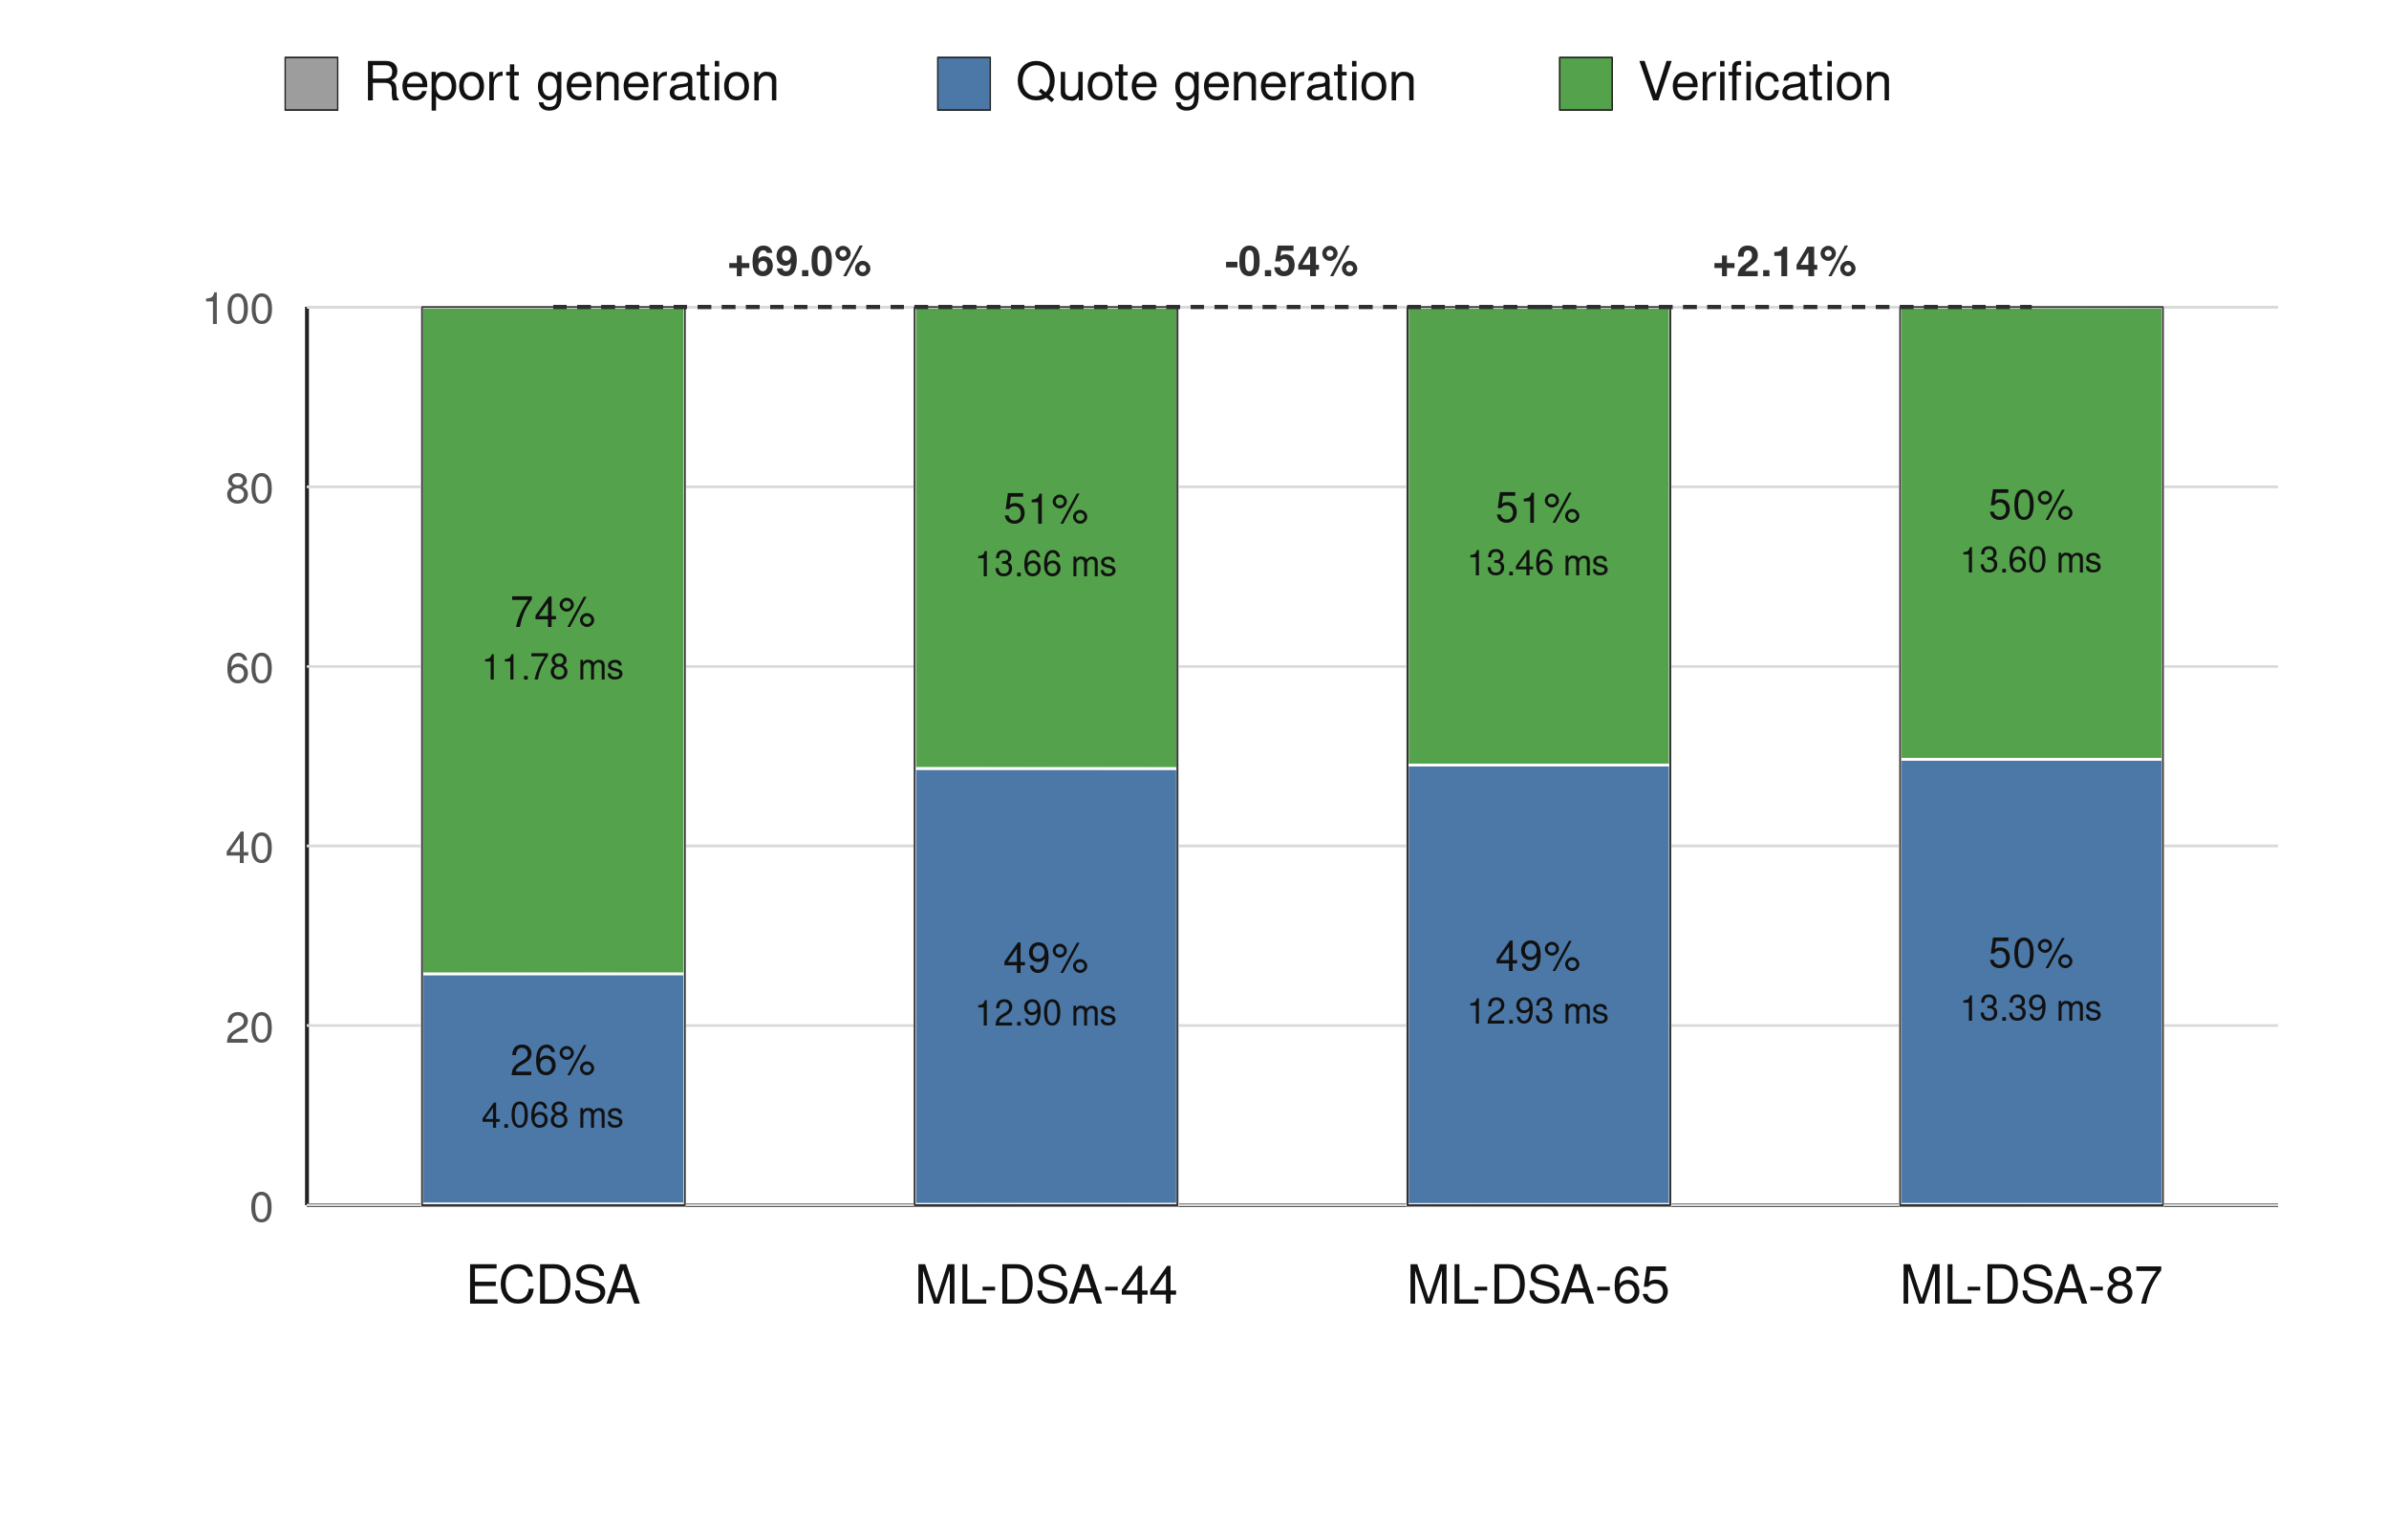
\includegraphics[width=0.90\linewidth]{figures/generated/end_to_end_stage_share_without_collateral.png}
\caption{Stage-share decomposition after removing the collateral-fetch stage.}
\label{fig:end-to-end-stage-share-without-collateral}
\end{figure}

\section{Discussion on Security-Performance Trade-offs}

The measured data support five main conclusions.

\begin{enumerate}
  \item \textbf{Reliability was stable in both measured contexts.} All direct
        attestation scenarios and all host-side prequote scenarios completed
        successfully in all 10 measured runs. All direct-path runs terminated
        with \texttt{qv\_ret=0} and \texttt{qv\_result=OK}. The experimental
        ML-DSA path therefore reached the same binary verification outcome as
        the stock ECDSA path in the tested configuration.

  \item \textbf{The quote-size cost of PQC is real and monotonic.} Moving from ECDSA to ML-DSA increased the direct quote size from 5006 B to 8847 B, 10376 B, and 12334 B for the 44, 65, and 87 parameter sets, respectively. This is the clearest direct security-performance trade-off exposed by the measurements: stronger parameter sets consume more bandwidth and enlarge the attestation evidence.

  \item \textbf{Collateral size is almost invariant.} The verifier-side collateral bundle remained essentially unchanged across all PQC runs. The marginal cost of the PQC scenarios therefore comes from the evidence object, not from the collateral payload.

  \item \textbf{Cryptographic runtime overhead is moderate.} The direct
        quote-generation stage increased by about \(3.17\times\) to
        \(3.29\times\) relative to ECDSA, while the direct verification stage
        rose by roughly \(1.14\times\) to \(1.16\times\). The runtime penalty
        is therefore significantly smaller than the dimensional penalty.

  \item \textbf{The end-to-end cost is dominated by trust-path plumbing in the present prototype.} The absolute end-to-end ML-DSA times were driven overwhelmingly by the collateral-fetch stage of the \texttt{local\_pcs\_tdqe\_identity} verifier path. This means that the current end-to-end penalty is not a pure function of the ML-DSA algorithm itself.
\end{enumerate}

For this reason, two levels of comparison should be kept distinct in the final
analysis. At the \textbf{algorithm level}, direct quote size, quote-generation latency,
and verification latency show the direct cost of replacing ECDSA with
ML-DSA. At the \textbf{system level}, end-to-end latency reflects not only the
signature algorithm but also the surrounding collateral and trust
infrastructure. The host-side prequote buffer-size measurements form a third,
separate category: they characterize wrapper-side allocation and control-path
behavior, not the final serialized evidence length.

Within the PQC family, ML-DSA-44 is the most economical option in terms of
direct quote size, while ML-DSA-65 and ML-DSA-87 increase the quote size
further without producing a proportionally larger quote-generation latency.
This indicates that, in the measured implementation, the choice among the
ML-DSA parameter sets is primarily a bandwidth and evidence-size decision,
whereas the dominant system-level latency cost lies in the verifier-side
collateral path. Stated differently, the present prototype exposes two
distinct trade-offs: if the design objective is to \textbf{minimize quote size and
transmission overhead while retaining a PQC signature algorithm}, \textbf{ML-DSA-44} is
the least expensive option among the tested variants; if the design objective
is to \textbf{maximize the cryptographic security margin}, \textbf{ML-DSA-87} provides the
strongest parameterization among the measured variants, at the price of the
largest attestation evidence.

ML-DSA-65 occupies the expected middle point: it offers an intermediate
security-performance compromise, with quote size and direct cryptographic cost
between the two extremes. In the current implementation, this middle position
is especially visible in the evidence size, while the direct \textbf{runtime gap
between ML-DSA-65 and ML-DSA-87 remains smaller} than the corresponding gap in
quote size.
